% Chapter 2

\chapter{Segmentation Neural Networks}

\lhead{Chapter 2. \emph{Segmentation Neural Networks}} % This is for the header on each page - perhaps a shortened title
\label{chp:cbct}
%----------------------------------------------------------------------------------------

\def\:{\hskip0pt} %Definisce un modo veloce per permettere a latex di sillabare correttamente anche parole come 4-connectivity. Il corretto utilizzo è il seguente: 4\:-\:connectivity.

% \section{Segmentation using Deep Neural Networks}
% \label{sec:segmentation}
% Today, deep neural netoworks are the state-of-the-art in many fields, including
% image segmentation. In this section, we will briefly review the most common
% approaches to segmentation using deep neural networks, and we will discuss the
% advantages and disadvantages of each approach.

% \subsection{Fully Convolutional Networks}
% \label{sec:fcn}
% Fully convolutional networks (FCNs) are a class of deep neural networks that
% are designed to perform pixel-wise classification. The main idea behind FCNs is
% to use a convolutional neural network (CNN) to extract features from the input
% image and return an output of the same size as the input image, where each
% pixel is assigned a class label. The main advantage of FCNs is that they can be
% trained end-to-end, which means that the network can be trained to perform the
% classification of each pixel without the need of any post-processing step. On
% the other hand, Deep Neural Networks lacks for explainability, which is a major
% drawback for medical applications.
% The architecture of such networks can be grouped as shown in Figure \ref{fig:fcn_architecture}.
% \begin{figure}[ht]
%   \centering
%   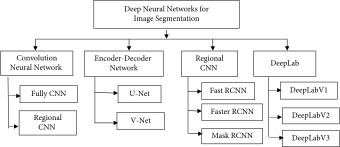
\includegraphics[width=0.8\linewidth]{Images/seg-arch.png}
%   \caption{Groups of a segmentation network architecture.}
%   \label{fig:fcn_architecture}
% \end{figure}

% \subsection{Convolutional Neural Networks}
% A convolutional neural network or CNN consists of a stack of
% three main neural layers: convolutional layer, pooling layer, and fully
% connected layer. Each layer has its own role. The convolution layer
% detects distinct features like edges or other visual elements in an image.
% Convolution layer performs mathematical operation of multiplication of local
% neighbours of an image pixel with kernels. CNN uses different kernels for
% convolving the given image for generating its feature maps. Pooling layer
% reduces the spatial \texttt{(width, height)} dimensions of the input data for the next
% layers of neural network. It does not change the depth of the data. This
% operation is called as subsampling. This size reduction decreases the
% computational requirements for upcoming layers. The fully connected layers
% perform high-level reasoning in NN. These layers integrate the various feature
% responses from the given input image so as to provide the final results.\\
% Different CNN models have been reported in the literature, including AlexNet,
% GoogleNet, VGG, Inception, SequeezeNet, and DenseNet. This type of networks were
% mostly used for classification, but they have been easily adapted to perform
% segmentation.

% \subsection{Fully Convolutional Networks}
% In fully convolutional network (FCN), only convolutional layers exist. The
% different existing in CNN architectures can be modified into FCN by converting
% the last fully connected layer of CNN into a fully convolutional layer. This
% type of networks can output spatial segmentation map and can have dense
% pixel-wise prediction from the input image of full size instead of performing
% patch-wise predictions. They can also uses skip connections, when performing upsampling
% on feature maps from final layer, these skip connections fuses it with the
% feature map of previous layers. The model thus produces a detailed segmentation
% in just one go but as drawback they do not have a global context of the image
% and the output can be fuzzy close to the boundaries of segmented objects.

% \subsection{Encoder-Decoder Networks}
% Encoder-decoder based models employ two-stage model to map data points from the
% input domain to the output domain. The encoder stage compresses the given input
% to a latent space representation, while the decoder predicts the output from
% this representation. This latent space representation is a compressed version of
% the input image, which is used to generate the output, it have smaller spatial dimension
% than the input image but an increased depth. In order to upsample this latent space representation
% to the size of the input image, transposed convolutional layers are used.
% One of the most popular encoder-decoder networks is the U-Net
% \cite{ronneberger2015u}, for which we can find in literature many variants. The
% U-Net architecture is shown in Figure \ref{fig:unet_architecture}.
% % \begin{figure}[ht]
% %   \centering
%   % \includegraphics[width=0.8\linewidth]{Images/unet-arch.png}
%   % \caption{U-Net architecture.}
%   % \label{fig:unet_architecture}
% % \end{figure}
% U-Net model has a downsampling and upsampling part. The downsampling
% section with FCN like architecture extracts features using $3 \times 3$ convolutions to
% capture context. The upsampling part performs deconvolution to decrease the
% number of computed feature maps. The feature maps generated by downsampling or
% contracting part are fed as input to upsampling part so as to avoid any loss of
% information. The symmetric upsampling part provides precise localization. The
% model generates a segmentation map which categorizes each pixel present in the
% image. This type of architecture proposed in 2015 is still widely used today as
% it can obtain state-of-the-art resuts.

% \subsection{Regional Convolutional Neural Networks}
% Regional convolutional network has been utilized for object detection and
% segmentation task. The R-CNN architecture presented in [69] generates region
% proposal network for bounding boxes using selective search process. These region
% proposals are then warped to standard squares and are forwarded to a CNN so as
% to generate feature vector map as output. The output dense layer consists of
% features extracted from the image and these features are then fed to
% classification algorithm so as to classify the objects lying within the region
% proposal network. The algorithm also predicts the offset values for increasing
% the precision level of the region proposal or bounding box. The processes
% performed in R-CNN architecture are shown in Figure 4. The use of basic RCN
% model is restricted due to the following:

% \subsection{DeepLab}
% DeepLab model employs pretrained CNN model ResNet-101/VGG-16 with atrous
% convolution to extract the features from an image. The use of atrous
% convolutions gives the following benefits:
% \begin{itemize}
%   \item{It controls the resolution of feature responses in CNNs}
%   \item{It converts image classification network into a dense feature extractor
%     without the requirement of learning of any more parameters employs
%     conditional random field (CRF) to produce fine segmented output}
% \end{itemize}
% The various variants of DeepLab have been proposed in the literature including
% DeepLabv1, DeepLabv2, DeepLabv3, and DeepLabv3+.
% In DeepLabv1, the input image is passed through deep CNN layer with one or
% two atrous convolution layers. This generates a coarse feature map. The feature
% map is then upsampled to the size of original image by using bilinear
% interpolation process. The interpolated data is applied to fully connect
% conditional random field to obtain the final segmented image.

\section{Supervised Learning}
In the medical image segmentation tasks, supervised learning is the most popular method, where the latests improvements mainly includes network backbones, network blocks and the design of novel loss functions.

\subsection{Backbone networks}
Encoder-decoder structure is the most popular end-to-end architectures, such
fully convolutional networks (FNC) like U-Net, Deeplab, and SegNet. The encoder
part aim to extract high level features from the input image and project them
into a latent space. The decoder part instead restore the extracted features
from the latent space to the original space size.

\subsubsection{U-Net and V-Net}
In 2015, Ronneberger et al.
proposed U-Net which has been widely used for medical image segmentation and
many variants have been proposed also in the recent years. The stucture of U-Net
is symmetrical and the main scope is to fuse low-level features, which medical
images are usually noisy but show blurred boundaries, with high level features
via skip connections.

U-Net was designed to deal with 2D images but when dealing with medical images,
we usually have to handle 3D images. A straighforward solution was to extract 2D
slices from the original image, fed them to the network and stack the outputs to
obtain the final 3D output.
The main drawback of this approach is that we lost the spatial information among
the slices as they are threated as independent images. Motivated by this idea,
Çiçek et al. proposed a solution to this problem by using 3D convolutions inside
U-Net. This network, named 3D U-Net, includes only three down-sampling steps
because of the high computational cost of 3D Convolutions, leading to a less
effective extraction of of deep-layer image features.
Milletari et al. proposed a similar architecture, named V-Net, which emply more
skip connections than U-Net to design a deeper network.
Some Recurrent Neural Network mixed with U-Net has been proposed to model the
time dependence of image sequences.

\subsubsection{Recurrent Neural Networks}
Gao et al. joined LSTM and CNN to model the temporal relationships between
different brain MRI slices to improve segmentation accuracy. Clearly, RNN can
capture local and global spatial features of images by considering the context
information
relationship. However, in medical image segmentation, the capture of complete
and valid temporal information requires good medical image quality (e.g. smaller
slice thickness and pixel spacing). Therefore, the design of RNN is uncommon for
improving the performance of medical image segmentation.

\subsubsection{Pseudo-3D Networks}
As stated before, most of the medical image are 3D images, but using 3D
convolution requires a lot of computational resources. Therefore some pseudo-3D
segmentation methods have been proposed. For example, Vu et al. applied the
overlay of adjacent slices as input to the centeral slice prediction and then
fed the obtained 2D feature map into a standar 2D network.

\subsubsection{Generative Adversarial Networks}
\label{subsubsec:gan}
Another type of networks that have been exploited in medical image segmentation are GANs, mostly for data augmentation by generating new samples. Pollastri et al. remodelled two different weel known GANs, Deep Convolutional GAN and a Laplacian GAN, to generate both skin lesion images and their segmentation masks, making the augmentation process extremely straighforward.
In addition, the incorporation of the prior knowledge about
organ shape and position may be crucial for improving medical
image segmentation effect, where images are corrupted and
thus contain artefacts due to limitations of imaging techniques.
However, there are few works about how to incorporate prior
knowledge into CNN models. As one of the earliest studies in this field, Oktay et al. proposed a novel and general
method to combine a priori knowledge of shape and label
structure into the anatomically constrained neural networks
(ACNN) for medical image analysis tasks. In this way, the neural network training process can be constrained and guided to
make more anatomical and meaningful predictions, especially
in cases where input image data is not sufficiently informative or consistent enough (e.g., missing object boundaries).\\

After proposing U-Net in [7], the encoder-decoder structure
became the most popular structure in medical image segmentation. The design of the network backbone focuses on more
efficient feature extraction in the encoder and feature recovery
and fusion in the decoder to improve segmentation accuracy.

\subsection{Network Function Block}
\subsubsection{Dense connection}
Dense connection is the most popular network block in medical image
segmentation, used to contruct a kin of special convolution neural networks. The
input of each layer comes from the output of all previous layers in the process
of forward transmission. Inspired by this design, Guan et al. proposed an
improved U-Net by replacing each sub-block of U-Net with a form of dense
connection. Although the dense connection is helpful for obtaining riher image
fetures, it often reduces the robustness of feature representation to a certian
extent and increase the number of parameters.

\subsubsection{Inception block}
For CNNs, deep networks often given better performances than shallow ones, buyt they encountr some new problems such as vanishing gradient, high memory usage, and slow convergence. The inception structure used in GoogleNet overcome this problems, and for this reason it has been also used over medical images. Gu et al. proposed CE-Net by introducing the inception structure and atrous convolution to each parallel structure to extrtact features on a wide reception field. Such complex structure however lead to a difficult model modification.

\subsubsection{Depth separability}
To reduce the computational cost of 3D convolutions and their memory usage,
Howard et al. proposed MobileNet to decompose vanilla convolutions into
depthwise separable convolution and pointwise convolution.
% TODO: aggiungere calcolo del numero di calcoli fatti tra le 3D e le depth
% separable

\subsubsection{Attention}
\par
Attention block can selectively change input or asssigns different weights to
input variables according to different importance.\\
\emph{Spatial Attention} block aims
to calculate the feature importance of each pixel in space-domain and extract
the key information of an image. Oktay et al. proposed attention U-Net, where
attention blocks were used to change the output of the encoder before fusing
features from the encoder and the corresponding decoder. The attention block
outputs a gating signal to control feature importance of pixels at different
spatial positions.\\
Another type of attention block is the \emph{Channel attention},
which utilizes learned global information to emphasize selectively useful
features and suppress useless features. Hu et al. proposed SE-Net that
introduced the channel attention to the field of image analysis and won the
ImageNet Challenge in 2017.\\
Spatial and channel attention mechanisms are the two most popular strategies for
improving feature representation. However, spatial attention ignores the
difference of different channel information and treats each channel equally. On
the contrary, the channel attention pools global information directly while
ignoring local information in each channel, which is a relatively rough
operation. Therefore, combining advantages of two attention mechanisms,
researchers have designed many models based on a \emph{mixed domain attention block}.

\subsection{Loss functions}
In addition to improved segmentation speed and accuracy
by designing network backbone and the function block, designing new loss functions also resulted in improvements in subsequent inference-time segmentation accuracy. Therefore,
a great deal of work has been reported about the design of
suitable loss functions for medical image segmentation tasks.

\subsubsection{Cross Entropy}
The cross entropy loss has been the most popular loss function. It compares pixel-wisely the predicted category vector with the real segmentation result vector and is defined as:
$$
L_{CE} = -\sum_{i=1}^{N} \sum_{j=1}^{C} y_{ij} \log \hat{y}_{ij}
$$
where $y_{ij}$ is the real segmentation result vector, $\hat{y}_{ij}$ is the
predicted segmentation result vector, $n$ is the number of pixels in the image,
and $C$ is the number of categories. The cross entropy loss is easy to
implement and has been widely used in medical image segmentation tasks. However,
it is not suitable for segmentation tasks with imbalanced data, because it does
not consider the class imbalance problem. Therefore, a \emph{weighted cross
entropy loss} and \emph{balanced cross entropy} have been proposed to solve this
problem, where a $\beta$ hyperparameters is added to the loss function to adjust
the weight of each class.

\subsubsection{Dice Loss}
The Dice coefficient is a popular metric for the evaluation of medical image segmentation tasks. This metric is the measure of overlap between a segmentation result and its corresponding ground thruth:
$$
DSC = \frac{2 \times |A \cap B|}{|A| + |B|}
$$
where $A$ and $B$ are the segmentation result and the ground truth, respectively. The \emph{Dice Loss} is then formulted as follow:
$$
L_{DSC} = 1 - \frac{2 \times y \times \hat{y} + 1}{y + \hat{y} + 1}
$$
Here 1 is added to the denominator to avoid the division by zero it the edge case when both $y$ and $\hat{y}$ are zero. The Dice loss is a good choice even for uneven samples, however it easly influences the back propagation and leads to a tranining difficulty.

\subsubsection{Generalized Dice Loss}
Although the Dice Loss can solve the problem of class imbalance to a certain extent, it does not work for serius class imbalance.
To solve this problem, researchers have proposed a \emph{Generalized Dice Loss} that can be used for both binary and multi-class segmentation tasks. The generalized Dice loss is defined as:
$$
L_{GDSC} = 1 - \frac{1}{m}\frac{2\sum_{j=1}^{m} \omega_j
\sum_{i=1}^{n}y_{ij}\hat{y}_{ij}}{\sum_{j=1}^{m}\omega_j\sum_{i=1}{n}(y_{ij} +
\hat{y}_{ij})}
$$
where the weight $\omega_j$ is used to adjust the weight of each class, and $\omega_j = 1/(\sum_{i=1}^{n}p_{ij})^2$.

\subsubsection{Boundary Loss}
Another approach to solve the problem of class imbalance have been proposed by Kervadec et al. for the task of brain lesion segmentation. They proposed a Boundary Loss which aims to minimize the distance between segmented boundaries and labeled boundaries. Results show that the combination of the Dice loss and the boundary loss is superior to the single ones. The composite loss is defined as:
$$
L = \alpha L_{DSC} + (1 - \alpha) L_{B}
$$
where the Boundary Loss $L_{B}$ for a binary segmentation is defined as:
$$
L_{B} = \sum \phi(y) \times \hat{y}
$$
where $\phi(y)$ is the signed distance function applied to the real segmentation $y$.

\par
For medical image segmentation, the improvement of loss mainly focuses on the
problem of segmentation of small objects in a large background (the problem of
class imbalance). Chen et al. proposed a new loss function by applying
traditional active contour energy minimization to convolutional neural networks,
Li et al. proposed a new regularization term to improve the crossentropy loss
function, and Karimi et al. proposed a loss function based on Hausdorff
distance (HD). Besides, there are still a lot of works trying to deal with this
problem by adding penalties to loss functions or changing the optimization
strategy according to specific tasks.\\
In many medical image segmentation tasks, there are often only one or two
targets in an image, and the pixel ratio of targets is sometimes small, which
makes network training difficult. Therefore, to improve network training and
segmentation accuracy, it is easier to focus on smaller targets by changing loss
functions than to change the network structure. However, the design of loss
functions is highly task-specific, so we need to analyze carefully task
requirement, and then design reasonable and available loss functions.

\section{Weakly Supervised and Unsupervised Segmentation}
Although convolutional neural networks show goods performances for medical
image segmentation, results seriously depend on high-quality
labels. In fact, it is rare to build many datasets with many high-quality labels,
especially in the field of medical image analysis, since data acquisition and
labeling often incur high costs. Therefore, a lot of studies on incomplete or
imperfect datasets are reported. Unsupervised learning is a very important
approach to improve the performance of medical image segmentation. In this
section, we will introduce the weakly supervised learning, a method which make
use of unsupervised learning for unlabelled data in combination with supervised
learning with labelled data.

\subsection{Data Augmentation}
Performing data augmentation is mandatory in absence of a largely labeled datasets, and is still considered a good practice even when we have enough data. However, new data generated with this method produce images that are highly correlated with the original images.

\subsubsection{Traditional methods}
With traditional methods we refer to all the computer vision techniques such as adding/removing noise, change brightness, saturation, contrast, colors, and change the image layout with rotations, distortion, scaling, etc. These technique are still very used today, usually combining them together with random parameters. Some of these algorithms may require a non negligible computational cost thus usually performed before the training procedure.

\subsubsection{Conditional Generative Adversarial Networks}
As already described in Section \ref{subsubsec:gan}, GAN and its variants have been widely for data augmentation. In particular, cGANs are often used in combination with standard GANs to generate labels relative to a given synthetic image.

\subsection{Transfer Learning}
Pre-trained model's parameters are often used to initialize a new model,
transfer learning can achieve fast training for data with limited labels. The
most popular approach is to use a model pretrained on ImageNet before performing
the training on the medical data. Experiments demonstrated that this approach is
useful as it improves the accuracy of segmentations. However the domain
adaptation may be a problem when applying models trained over natural images to
medical images analysis tasks. Moreover, these methods are hardly applicable to
3D medical image analysis because such pre-trained model rely on 2D datasets.\\
Hatamizadeh et al. recently proposed an unsupervised approach to pre-train a
given model by relying only on unannotated medical images of the same domain of
the main tasks. In pratice, the network is trained to perform a variety of tasks
such as image reconstruction, classification of the rotation applied to the
original image, etc. which can be performed in an unsupervised manner. Later,
these tasks heads of the network are detached and the training on the main task
is performed. Such pretraining aim to train the network to learn how to extract
high level feature from a specific type of medical images, such as CT or MRI.\\
Also Cipriano et al. recently proposed a pre-training approach based on sparse labels.
This type of labels are way easier to obtain but are not as accurate as the
real dense labels. They fed these labels to the network together with the input
image for a given number of steps, then used the learned parameters to train the
network to produce the segmentation by relying only on the input, without the
sparse labels.


\section{Current direction of research}
Until now we described the most popular network structures and loss functions
for medical image segmentation tasks that were proposed and used up to date.
Since the raise in popularity of vision transformers and graph neural networks,
some novelty architectures are being proposed in medical imaging. Results
obtained are still not as good as those obtained with traditional architectures,
aside some really specific tasks or datasets, but they are still interesting and
promising.\\

\subsection{Network Architecture Search}
The design process of a network architecture is a very time consuming task, and
it is often difficult to find the best architecture for a given task. Therefore,
many researchers have proposed methods to automate the design of network
architectures. Such methods, named NAS (Network Architecture Search), focus on
the \emph{search space}, \emph{search strategy}, and \emph{performance
estimation}.
The search space is a candidate collection of network structures to be searched.
The search space is divided into a global search space that represents the
search for the entire network structure, and a cell-based search space that
searches only a few small structures that are assembled into a complete large
network by the ways of stacking and stitching. The search strategy aims to find
the optimal network structure as fast as possible in search spaces. Popular
search strategies are often grouped into three categories, reinforcement-based
learning, evolutionary algorithms, and gradients. Performance estimation
strategy is the process of assessing how well the network structure performs on
target datasets. For NAS techniques, researcher pay more attention to the
improvement of search strategies since search space and performance estimation
methods are usually rarely changed.\\
Isensee et al. argued that too much manual adjustment on network structure could
lead to over-fitting for a given dataset, and therefore proposed a medical image
segmentation framework no-newUNet (nnU-Net) that adapts itself to any new
dataset. The nnUnet automatically adjusts all hyperparameters according to the
properties of the given dataset without manual intervention. Therefore, the
nnU-Net only relies on vanilla 2D UNet, 3D UNet, UNet cascade and a robust
training scheme. It focuses on the stage of pre-processing (resampling and
normalization), training (loss, optimizer settings, data augmentation),
inference (patch-based strategies, test-time-augmentations integration, model
integration, etc.), and post-processing (e.g., enhanced single pass domain). In
practical applications, the improvements of network structure design usually
depend on experiences without adequate interpretability theory support,
Moreover, more complex network models indicate higher risk of over-fitting.


\subsection{Graph Convolutional Neural Network}
Graph Convolutional Neural Network (GCN) is a type of neural network that
utilizes graph structure to process data. In practive the Euclidean space of the
image can be converted into graphs that can be modeled using GCN.

Gao et al. designed a new graph pooling (gPool) and graph unpooling (gUnpool)
operation based on GCN and proposed an encoder-decoder model namely graph U-Net.
The graph U-Net achieves better performance than popular UNets by adding a small
number of parameters. In contrast to traditional convolutional neural networks
where deeper is better, the performance of the graph U-Net cannot be improved by
increasing the depth of networks when the value of depth exceeds 4. However, the
graph U-Net show stronger capability of feature encoding than popular U-Nets
when the value of depth is smaller or equivalent to 4.

Yang et al. proposed the end-to-end conditional partial residual plot
convolutional network CPR-GCN for automatic anatomical marking of coronary
arteries. Authors showed that the GCN-based approach provided better performance
and stronger robustness than traditional and recent depth learning based
approaches. Results from these GCNs in medical image segmentations are
promising, as the graph structure has high data representation efficiency and
strong capability of feature encoding

\subsection{Interpretable Shape Attentive Neural Network}
Currently, many deep learning algorithms tend to make judgments by using
"memorized`` models that approximately fit to input data. As a result, these
algorithms cannot be explained sufficiently and give convincing evidences for
each specific prediction. Therefore, the study of the interpretability of deep
neural networks is a hot topic at present. Sun et al. proposed the SAU-Net that
focuses on the interpretability and the robustness of models. The proposed
architecture attempts to address the problem of poor edge segmentation accuracy
in medical images by using a secondary shape stream. Specially, the shape stream
and the regular texture stream can capture rich shape-dependent information in
parallel. Furthermore, both spatial and channel attention mechanism are used for
the decoder to explain the learning capability of models at each resolution of
U-Net. Finally, by extracting the learned shape and spatial attention maps, we
can interpret the highly activated regions of each decoder block. The learned
shape maps can be used to infer correct shapes of interesting categories learned
by the model. The SAU-Net is able to learn robust shape features of objects via
the gated shape stream, and is also more interpretable than previous works via
built-in saliency maps using attention.

\subsection{Vision Transformer}
Recently, transformer-based architectures have become very popular that replaces
the convolutional operator and use self-attention modules to compose entire
encoderdecoder structures that can encode long-range dependencies.
It has been a great success in the field of natural language processing.
Dosovitskiy et al. proposed Vision Transformer (ViT) that is able to classify
images directly using the Transformer.
Recently, a large number of researches have applied the transformer to medical
image segmentation. CNNs have a comparative advantage in extracting the
underlying features. These low-level features form the key points, lines, and
some basic image structures at the patch level. However, when we detect these
basic visual elements, the higher-level visual semantic information is often
more concerned with how these elements relate to each other to form an object,
and how the spatial location of objects relates to each other to form the scene.
At present, the transformer is more natural and effective in dealing with the
relationships between these elements. However, if all the convolutional
operators in CV tasks are replaced by Transformer, it may suffer from many
problems, such as high computational cost and memory usage. From existing
researches, the combination of Transformer and CNNs may lead to better results.
Recently, Chen et al. proposed a U-Net shaped network, where the encoder was
made of ViT only while the decoder was fully convolutional.



% \section{Dealing with 3D Medical Images}
% It is not uncommon in the medical field to deal with 3D images that comes from
% CT scans or MRI scans. In this case, a 3D image can be represented as a stack of
% 2D images and fed them to the network. Each output is then stacked back to
% produce the final 3D output. Another approach is to use 3D convolutional
% networks. The 3D convolutional network is a generalization of the 2D
% convolutional network to 3D data.
% In the first case, each 2D layer is indipendend from the others, while in the
% second case, the 3D convolutional network is able to learn the spatial
% relationships between the different slices of the 3D image.
% However, these 3D CNN architectures come with high computational overheads due
% to multiple layers of 3D convolutions, which may make these models prohibitive
% for practical large-scale applications. In order to overcome these problems, pseudo-3D
% CNN have been proposed in the literature. These models apply 2D convolutions on
% both the direction of the slices and the depth of the 3D image. This approach
% is able to reduce the computational overheads of the 3D CNNs while still
% preserving the spatial relationships between the slices of the 3D image.


